\documentclass[a4paper, textwidth=18cm, textheight=24cm, top=1cm, bottom=1cm, left=1cm, right=1cm10pt]{article}
% File icdp2009.sty
% Preamble that you have to include to use the template  

% July 24, 2009
% Contact: simonnet@ecole.ensicaen.fr

\usepackage[a4paper, textwidth=18cm, textheight=24cm, top=1.5cm, bottom=2.85cm, left=1.5cm, right=1.5cm]{geometry}

\usepackage{template/icdp2009}

% left justified caption
\makeatletter
\long\def\@makecaption#1#2{%
\vskip\abovecaptionskip
\sbox\@tempboxa{#1. #2}%
\ifdim \wd\@tempboxa >\hsize
#1. #2\par
\else
\global \@minipagefalse
\hb@xt@\hsize{\box\@tempboxa\hfil}%
\fi
\vskip\belowcaptionskip}
\makeatother




%other package
\usepackage{lmodern}
\usepackage{graphicx}
\usepackage{times}
\usepackage{enumitem}
\usepackage{hyperref}
\usepackage{xcolor}

\begin{document}
\noindent

\bibliographystyle{plain}

\title{Space-time volumes for classification of platform diving tricks}

\authorname{C. Lenzenweger, B. Sespede}

\maketitle

\section{Topic and data}

In this KU we trained a support vector machine (SVM) in order to classify video recordings of different styles of platform diving. In platform diving the performances are composed by three main stages: takeoff, flight, and entry. The flight stage is the one where the diver is in air and can be sub-classified into three distinct types as shown in Figure \ref{fig:dive-styles} (and a fourth "free" style composed by a combination of the other three). During the jump, the performer is expected to do somersaults using these positions. Furthermore, the diver might perform twists when switching between styles in a single dive.

\begin{figure}[!htb]
\center{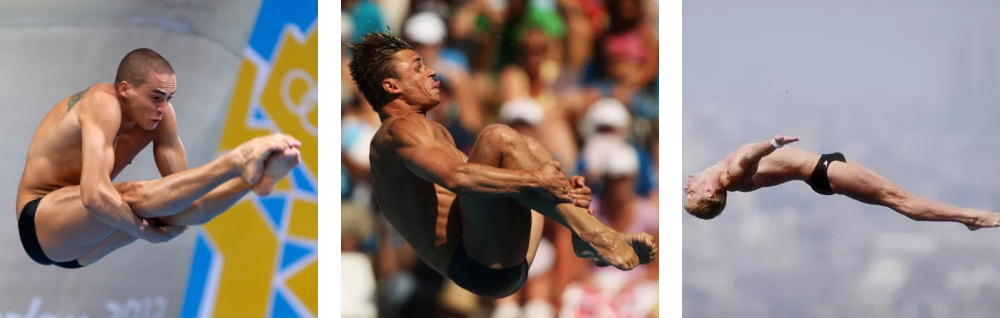
\includegraphics[scale=0.98]
{figures/dives.png}}
\caption{\label{fig:dive-styles} The figure shows the three main flight styles from left to right: pike, tuck, and straight.}
\end{figure}

Our goal was to extract meaningful features from space-time volumes (STVs) in order to train an SVM. The SVM was then be used to classify the three different flight styles in previously unseen videos (styles shown in Figure~\ref{fig:dive-styles}). To train our SVM we used the \textit{Diving48} dataset \cite{ref-diving48} which contains a large number of recordings from a variety of angles. To simplify the extent of our work we decided to make certain restrictions to the original dataset. First, we removed the "free" flight style from the dataset (i.e. the style where the performer combines several styles in one dive). Furthermore, we cropped the recordings to remove the parts where the performer sinks below the water, as the STVs of nearby frames break when doing so. Furthermore, we removed the performances with extreme camera angles and twists in them. The intention behind these modifications was to allow us to focus exclusively on flight style classification while keeping it challenging enough.

Upon further analysis of the dataset we discovered several issues that needed to be solved. First, the quality of the videos was not consistent, while some videos contained a lot of motion blur, some did not. When we first computed the STVs on a naive selection of videos we noticed that this had a direct impact on the quality of our feature extraction. As a second issue, the ground-truth labels provided by the authors of the dataset were not accurate, so we needed to make our own annotations in order to reliably train our SVM. With these ideas in mind, we implemented an annotation tool capable of cropping the videos to time slots were the flight style was clearly visible, and with which we could quickly indicate the flight style of the video. Using the tool, we made a selection of 100 high-quality cropped videos per flight style (300 in total).

Once we had chosen appropriate videos, Filip Illic kindly provided us with the corresponding STVs. Upon a quick visual analysis we noticed that not all of the videos were fit for feature extraction since many of them contained either strong artifacts or no STVs at all (sample artifacts shown in Figure~\ref{fig:artefacts}). Considering that feature extraction would be inaccurate in such videos, we had to narrow down our original selection to 113 videos in total. During such selection, we took special care to choose a selection of videos (approximately 38 videos per flight style).

\begin{figure}[!htb]
\center{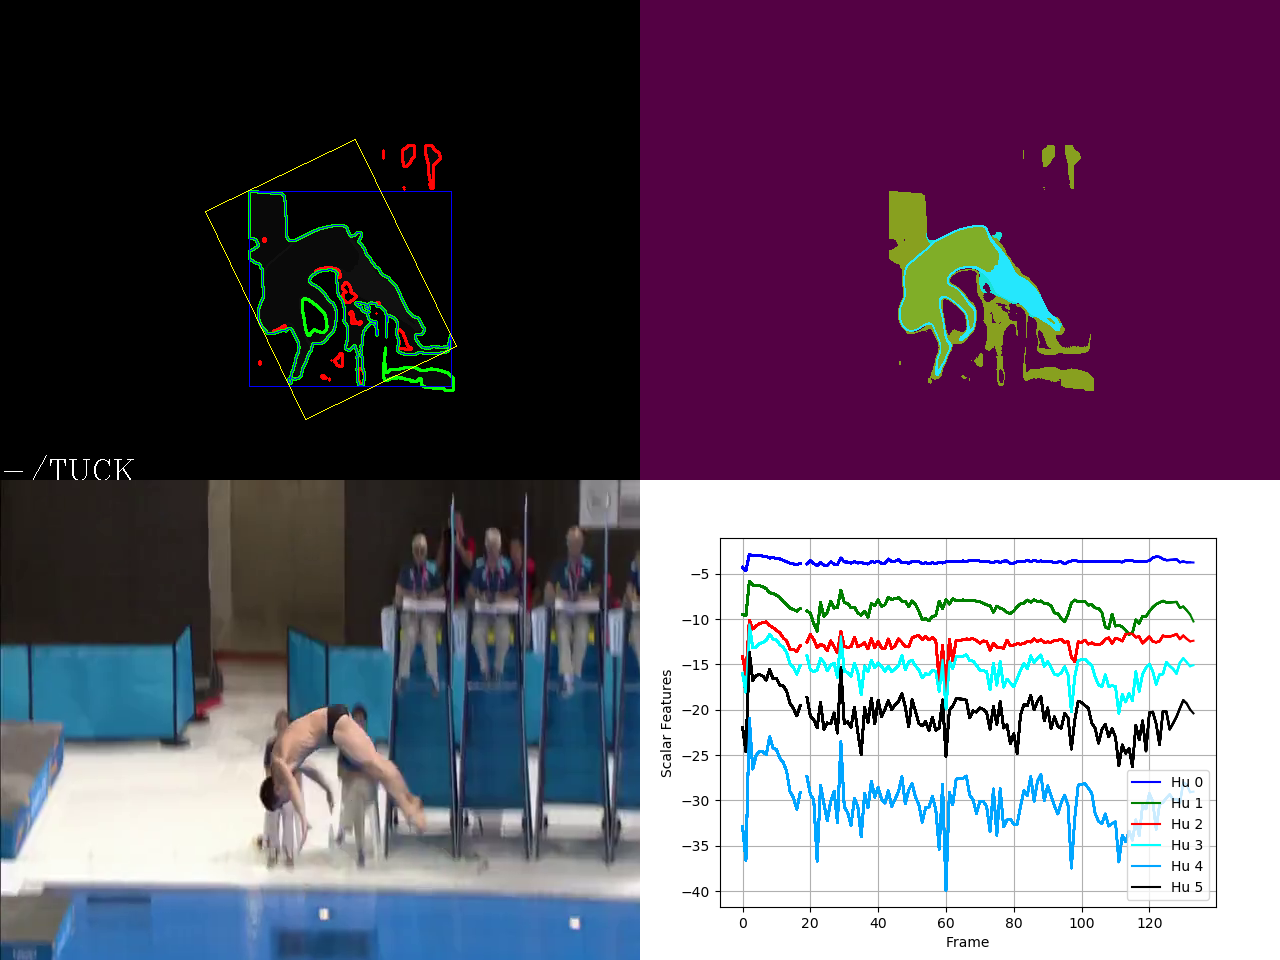
\includegraphics[scale=0.31]
{figures/tuck_artefacts1.png}}
\caption{\label{fig:artefacts} Illustration of STV occasional artefacts. Top-left: rejected (red) and selected (green) STV contours and bounding box for further feature extraction. Top-right: STVs with identifier as false color. Bottom-left: original RGB frame. Bottom-right: extracted (yet unfiltered) features of current and previous frames.}
\end{figure}

\section{Proposed solution}

In order to solve this problem we propose the following pipeline using the \emph{OpenCV} library in Python:

\textbf{Extraction of STVs and Pre-processing.} In this step Filip Illic provided us with three-dimensional tensors containing the STVs, and other relevant data such as optical flow estimation. Considering the algorithm for STV extraction can introduce artifacts from the background when the camera is moving, we decided to perform certain operations per frame to improve the accuracy of upcoming feature extraction: (i) we find the three contours with the largest area enclosing contiguous - but potentially different - STVs (as they usually represent the diver), (ii) from these contours we remove those which either have a relative area less than two thirds of the largest one (as these are usually spurious background artefacts) or are enclosing less than two third of the STVs (distinguished by the unique STV ID) of the largest one, (iii) and finally merge them into one binary mask. Using this mask, we compute the set of scalar features.

\textbf{Feature Extraction and Token Selection.} In an ideal setting the token list should represent the pose of the diver completely. To this end, we considered several features that could describe, quantify, and characterize the pose of the diver in a translation, scale and rotation invariant manner. We had initially considered fitting ellipses and to extract information about the rotation and center of mass of the diver within a minimum bounding rectangle, but then realized that most of these features could be superseded by the use of normalized Hu invariant moments \cite{hu62}. Furthermore, we found out that the STVs describing the diver would sometimes separate into multiple disjoint masks making fitting primitives an unreliable approach. 

\textbf{Pre-processing in Feature Space.} Since some of the videos were horizontally reflected we skipped the 7th Hu, which is not reflection invariant by definition. Analysis of the actually extracted features showed, that some moments flip sign on some isolated frames. Thus, their absolute value is taken. Besides, the natural logarithm was taken in order to have the individual moments in a comparable range of magnitude. Finally, we reduce the influence of artefact noise and STV flickering by temporally filtering the resulting features using a median filter over a window of 9 frames.

\textbf{Classification.} As mentioned in the introduction, the actual classification was performed by training an SVM. The specific implementation used was the one provided by \emph{OpenCV}. In particular, we used the SVM training method which automatically chooses the hyper-parameters by picking values that minimizes the test set error by means of a cross-validation estimate. Choosing a multi-class $\nu$-SVM with radial basis functions (RBF) as kernels, provided best classification accuracy.

When it comes to training, we used the pre-processed STV to extract the corresponding Hu moment, along with the manually annotated label of the flight style for the video, and used them as a training sample for the SVM. We repeated this process for each frame of the selected videos. 
As a main topic of this project, we wanted to evaluate the impact of aggregating temporal data versus classifying in a frame-wise manner, so we evaluated the following training approaches:
\begin{enumerate}[nosep]
\item \emph{Frame-wise scheme}: Once the SVM is trained, we predict the label for each individual frame and report accuracy result in a frame-wise manner.
\item \emph{Frame-voting scheme}: In this case, we chose to use a voting scheme in which every frame predicts a label and the final classification result for a video corresponds to the most voted label. With this approach we wanted to minimize the impact of miss-classifications due to broken STVs in some frames. 
\end{enumerate}

\section{Results}

In order to evaluate the proposed solution, and considering we only had a limited number of training/testing videos, we decided to perform several runs while randomly choosing videos from the train/test set using a 90/10 split. In Figure~\ref{fig:box_class} we show the frame-wise and video-wise classification accuracy after executing our algorithm one hundred times on the randomized (i.e. randomly shuffled frames) data. The classification accuracy of the straight pose is apparently worse due to the unbalanced dataset (i.e. fewer straight data).

\begin{figure}[!htb]
\center{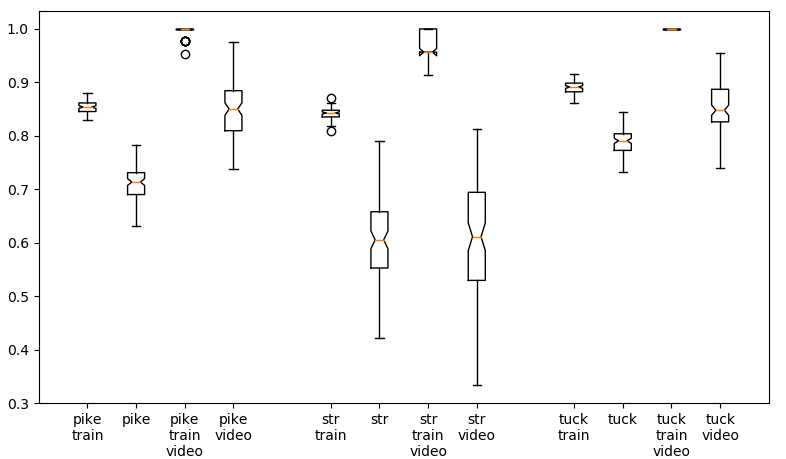
\includegraphics[scale=0.45]
{figures/box_class.png}}
\caption{\label{fig:box_class} Box plot of the classification result using the frame-wise scheme (100 runs).}
\end{figure}

Beyond the classification accuracy, we decided to compute the corresponding confusion matrices for each of the labels, in order to understand possible sources of miss-classification. Finally, to visually inspect the feature space, we plotted the value of the Hu moments over time.

\begin{table}[!htb]
    \centering
    \begin{tabular}{c|c|c|c}
         true $\backslash$ predicted & Pike & Straight & Tuck\\
         \hline \hline
         Pike&    121.14&    3.64&  46.22\\
         \hline
         Straight&  7.33&  23.2&   7.47\\
         \hline
          Tuck&    53.64&    3.48& 207.88
    \end{tabular}
    \caption{Mean (100 runs) confusion matrix for frame-wise classification. Rows represent true class. Columns represent predicted class.}
    \label{tab:confusion_matrix_frame}
\end{table}

\begin{table}[!htb]
    \centering
    \begin{tabular}{c|c|c|c}
         true $\backslash$ predicted & Pike & Straight & Tuck\\
         \hline \hline
         Pike&    33.84&    0.38&  5.5\\
         \hline
         Straight&  4.73&  11.11&   2.37\\
         \hline
          Tuck&    6.74&    0.14& 38.8
          
    \end{tabular}
    \caption{Mean (100 runs) confusion matrix for video-wise classification. Rows represent true class. Columns represent predicted class.}
    \label{tab:confusion_matrix_video}
\end{table}

\section{Discussion}

Upon further inspection of the confusion matrix, we noticed that the \emph{pike} and \emph{tuck} tend to get confused for each other, as these are the styles who are most physically similar. As shown in Figure~\ref{fig:pike_as_tuck} we've noticed that the STVs for the \emph{pike} get usually separated into two parts, one for the legs and another for the chest/head. As shown in the figure, the chest usually looks like a diver in \emph{tuck} position, introducing classification inaccuracies into our algorithm. These results are congruent with the accuracy's obtained for each of the classes.

\begin{figure}[!htb]
\center{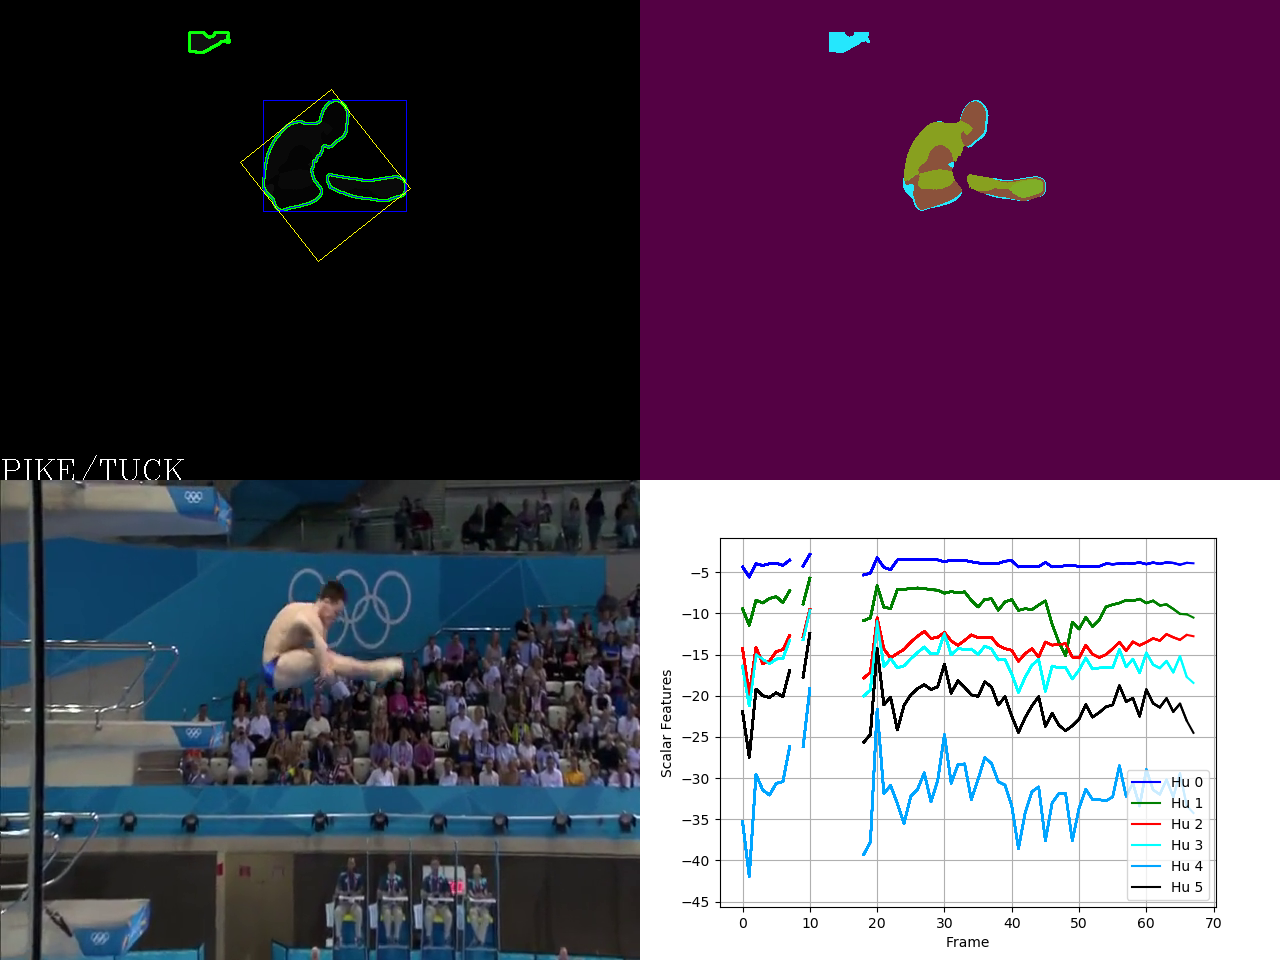
\includegraphics[scale=0.31]
{figures/pike_as_tuck3.png}}
\caption{\label{fig:pike_as_tuck} Confusion of the actual pike pose with the tuck pose due to separated STV.}
\end{figure}

When it comes to STVs themselves, we noticed they are not ideally suited for our problem, since the STV extraction breaks down when there is predominantly rotational motion. Furthermore, STVs are quiet sensitive to the quality of the input video. This implied that we had to make a careful selection of videos to be able to obtain meaningful results. Another source of error when it comes to STVs, is the fact they are not always temporally consistent, showing good results in a few frames and breaking down at a later time in the same videos. This made it specially hard to choose appropriate videos for our problem.

Two adaptions which significantly improved classification accuracy shall be mentioned: Firstly, the individual median filtering over time in feature space, which helps to further reduce the amount of artefacts fed to the SVM. Secondly, the temporal aggregation of the frame-wise classification results, which reduces the amount of frames with broken/flickering STVs.

The chosen conventional machine learning approach (using SVMs) appeared to be a reasonable choice for this task, when considering the resulting video classification accuracy. However, training a convolutional neural network (CNN), being capable to gain further expressiveness from the frame sequence, might improve the performance. However, this would require significantly more labeled video data compared to the frame-wise processing.

When it comes to features, we've noticed the potential of using orientation invariant Hu moments as a shape descriptor. In our particular case, this proved particularly useful since the poses a diver can take are standardized, thus making the problem easier.

\section{Conclusion}

After completing this project, we've shown a potential pipeline for classification of diving performances. We've concluded that STVs are not particularly reliable for the problem we are trying to solve due to rotational movement during somersaults. When it comes to features, we discovered that Hu moments are particularly suitable. In a further work it could be interesting to explore CNNs, as they might learn other features that we did not explore in our work (e.g. that divers wear swimsuits, or that humans have faces and connected limbs).

\bibliography{references/references.bib}

\end{document}